\documentclass[12pt]{article}
\usepackage[english]{babel}
\usepackage[utf8]{inputenc}

%% Pointer to 'default' preamble
% pacakages and definitions

\usepackage{geometry}
\geometry{
	letterpaper, 
	portrait, 
	top=.75in,
	left=.8in,
	right=.75in,
	bottom=.5in		} 	% Page Margins
	
%% additional packages for nice things
\usepackage{amsmath} 	% for most math
\usepackage{commath} 	% for abs
\usepackage{lastpage}	% for page count
\usepackage{amssymb} 	% for therefore
\usepackage{graphicx} 	% for image handling
\usepackage{wrapfig} 	% wrap figures
\usepackage[none]{hyphenat} % for no hyphenations
\usepackage{array} 		% for >{} column characterisctis
\usepackage{physics} 	% for easier derivative \dv....
\usepackage{tikz} 		% for graphic@!
\usepackage{circuitikz} % for circuits!
\usetikzlibrary{arrows.meta} % for loads
\usepackage[thicklines]{cancel}	% for cancels
\usepackage{xcolor}		% for color cancels
\usepackage[per-mode=fraction]{siunitx} % for si units and num
\sisetup{group-separator = {,}, group-minimum-digits = 3} % additional si unit table functionality

\usepackage{fancyhdr} 	% for header
\usepackage{comment}	% for ability to comment out large sections
\usepackage{multicol}	% for multiple columns using multicols
\usepackage[framed,numbered]{matlab-prettifier} % matlab sytle listing
\usepackage{marvosym} 	% for boltsymbol lightning
\usepackage{pdflscape} 	% for various landscape pages in portrait docs.
%\usepackage{float}
\usepackage{fancyvrb}	% for Verbatim (a tab respecting verbatim)
\usepackage{enumitem}	% for [resume] functionality of enumerate
\usepackage{spreadtab} 	% for using formulas in tables}
\usepackage{numprint}	% for number format in spread tab
\usepackage{subcaption} % for subfigures with captions
\usepackage[normalem]{ulem} % for strike through sout

% for row colors in tables....
\usepackage{color, colortbl}
\definecolor{G1}{gray}{0.9}
\definecolor{G2}{rgb}{1,0.88,1}%{gray}{0.6}
\definecolor{G3}{rgb}{0.88,1,1}

% For table formatting
\usepackage{booktabs}
\renewcommand{\arraystretch}{1.2}
\usepackage{floatrow}
\floatsetup[table]{capposition=top} % put table captions on top of tables

% Caption formating footnotesize ~ 10 pt in a 12 pt document
\usepackage[font={small}]{caption}

%% package config 
\sisetup{output-exponent-marker=\ensuremath{\mathrm{E}}} % for engineer E
\renewcommand{\CancelColor}{\color{red}}	% for color cancels
\lstset{aboveskip=2pt,belowskip=2pt} % for more compact table
%\arraycolsep=1.4pt\def
\setlength{\parindent}{0cm} % Remove indentation from paragraphs
\setlength{\columnsep}{0.5cm}
\lstset{
	style      = Matlab-editor,
	basicstyle = \ttfamily\footnotesize, % if you want to use Courier - not really used?
}
\renewcommand*{\pd}[3][]{\ensuremath{\dfrac{\partial^{#1} #2}{\partial #3}}} % for larger pd fracs
\renewcommand{\real}[1]{\mathbb{R}\left\{ #1 \right\}}	% for REAL symbol
\newcommand{\imag}[1]{\mathbb{I}\left\{ #1 \right\}}	% for IMAG symbol
\definecolor{m}{rgb}{1,0,1}	% for MATLAB matching magenta
	
%% custom macros
\newcommand\numberthis{\addtocounter{equation}{1}\tag{\theequation}} % for simple \numberthis command

\newcommand{\equal}{=} % so circuitikz can have an = in the labels
\newcolumntype{L}[1]{>{\raggedright\let\newline\\\arraybackslash\hspace{0pt}}m{#1}}
\newcolumntype{C}[1]{>{\centering\let\newline\\\arraybackslash\hspace{0pt}}m{#1}}
\newcolumntype{R}[1]{>{\raggedleft\let\newline\\\arraybackslash\hspace{0pt}}m{#1}}

%% Header
\pagestyle{fancy} % for header stuffs
\fancyhf{}
% spacing
\headheight 29 pt
\headsep 6 pt

%% Header
\rhead{Thad Haines \\ Page \thepage\ of \pageref{LastPage}}
\chead{Refined `Un-Trip' Results \\  }
\lhead{Research \\ 08/31/20}

\usepackage[hidelinks]{hyperref} % allow links in pdf
\usepackage{setspace}
\usepackage{multicol}
\usepackage{lscape}
\usepackage{minted}

\begin{document}
\onehalfspacing

\paragraph{Test System}\ A simple 3 machine system was used for `un-trip' testing.
All machines were modeled with governors, exciters, and PSS.
Most model parameters are the same, with the exception of MVA base.
Generators 1, 2, and 3, have an $M_{base}$ of 500, 200, and 100 MVA respectively. \\
The experimental goal was to trip Generator 3 off-line, and then `nicely' re-connect it.

\begin{center}
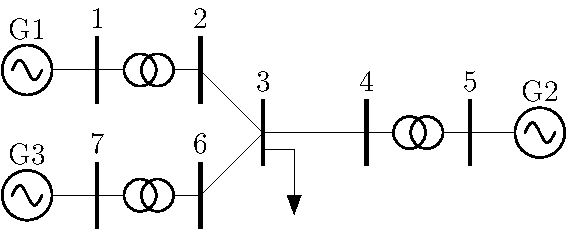
\includegraphics[width=.6\linewidth]{200831-3mach7bus}
\end{center}

\paragraph{Test Event Time Line:}
\begin{itemize}
\itemsep 0 em
\item $t=0$ - System initialized
\item $t=5$ - Generator 3 trips off.
Associated derivatives, $P_{mech}$, and governor $P_{ref}$ set to zero.
\item $t=15$ - Generator 3 re-synced to system and infinite reactance reset to original value. 
Negative Q flow between buss 6-3 is observed.
\item $t=20-25$ - The governor attached to Generator 3 is reinitialized and the $R$ value is ramped to its original value. 
This causes some mechanical power to be generated by Generator 3 which causes minor transients in system machine speed.
\item $t=35$ - The exciter on generator 3 is re-initialized and the bypass is removed.
This causes more reactive power flow into generator 3, the attached bus voltages to decrease, and system speed to increase. 
\item $t=45-65$ - Ramping the governor $P_{ref}$ to the original value increases system speed  and real power flow from Generator 3.
\item $t=80-100$ - Ramping exciter reference voltage to original its value decreases system speed and increases reactive power flow from generator 3.
\item $t=150$ - Simulation End
\end{itemize}

\paragraph{Observations of Note:}
\begin{itemize}
%\item The re-connected speed of Generator 3 was set to match Generator 1.
%\item The ramping of R causes a minor 
%\item The exciter was not being initialized to the correct reference voltage time index (i.e. \verb|g.exc.exc_pot(x,3)| referenced index 1 instead of $k$ ). This has been resolved however the exciter still produces a transient when it is bypassed.
\item Nicely `un-tripping' a generator seems pretty possible.
\item Generator 3 power does not return to set $P_{ref}$ value of 0.5 PU.
\item Exciter transient caused by bypass removal seems tricky to avoid.\\
Should probably be reinitialized and enabled at the same time as generator un-trip.
\item Scenario development using FTS as VTS will likely present additional reinitialization issues.
\end{itemize}

\pagebreak
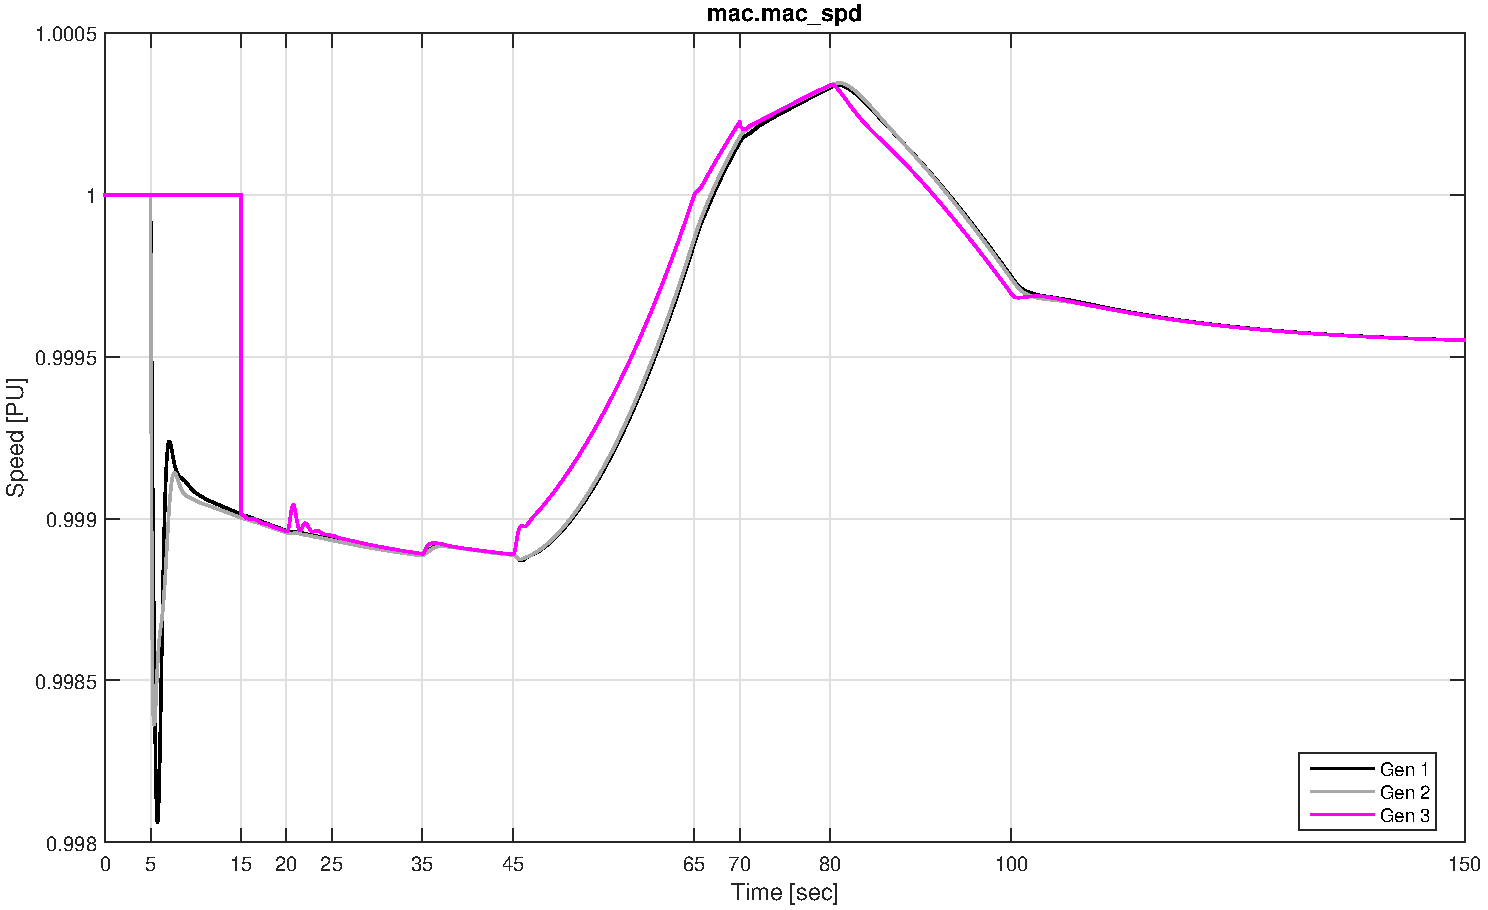
\includegraphics[width=\linewidth]{distinctSpeed}
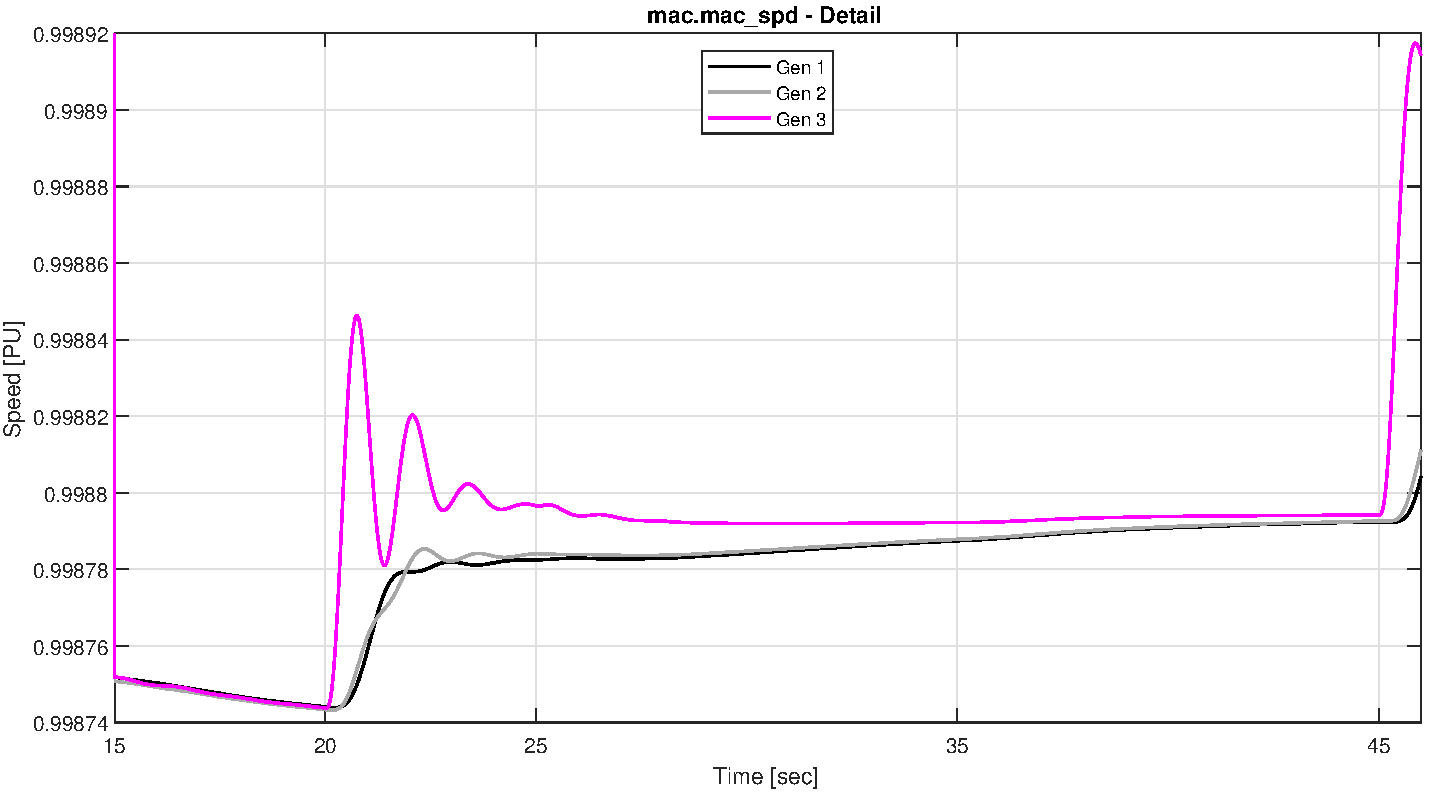
\includegraphics[width=\linewidth]{distinctSpeedDetail}


\pagebreak
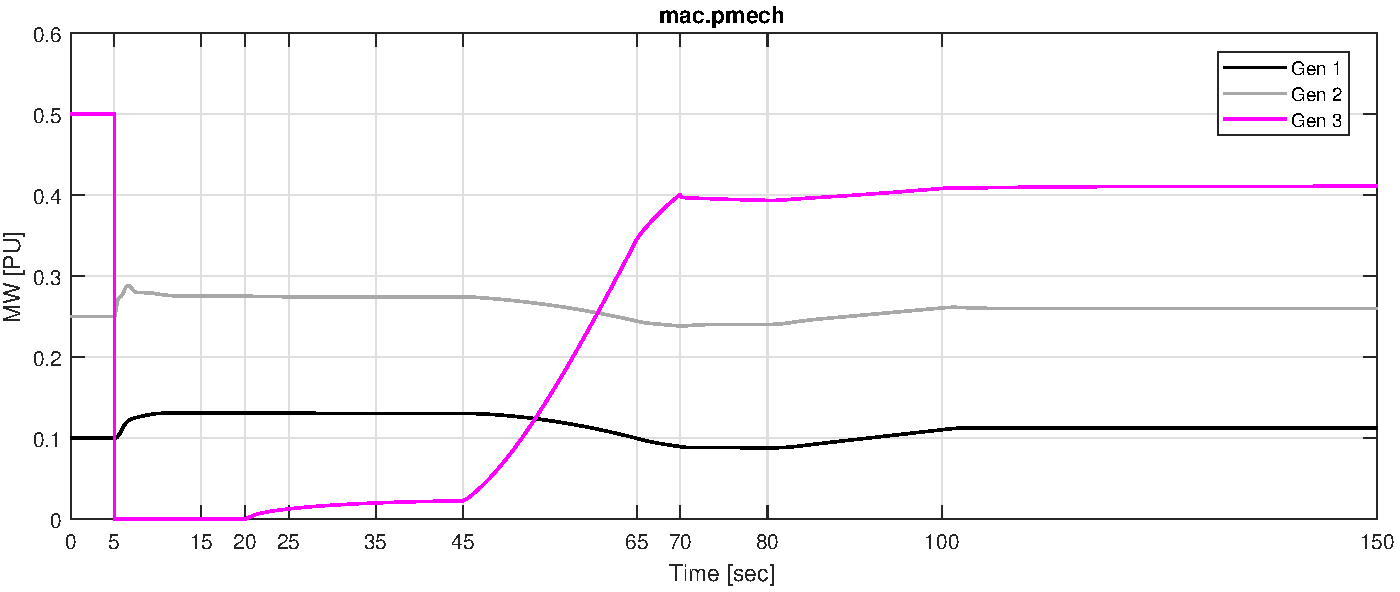
\includegraphics[width=\linewidth]{distinctPmech}
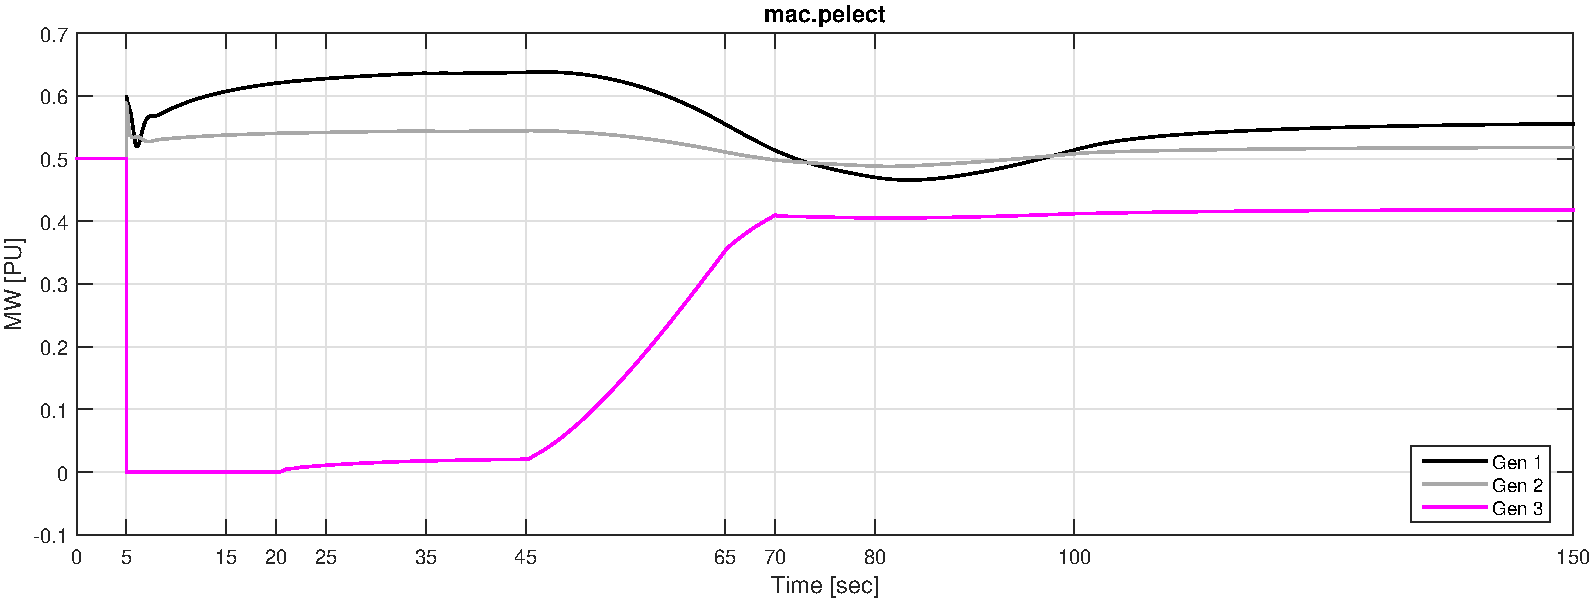
\includegraphics[width=\linewidth]{distinctPelect}
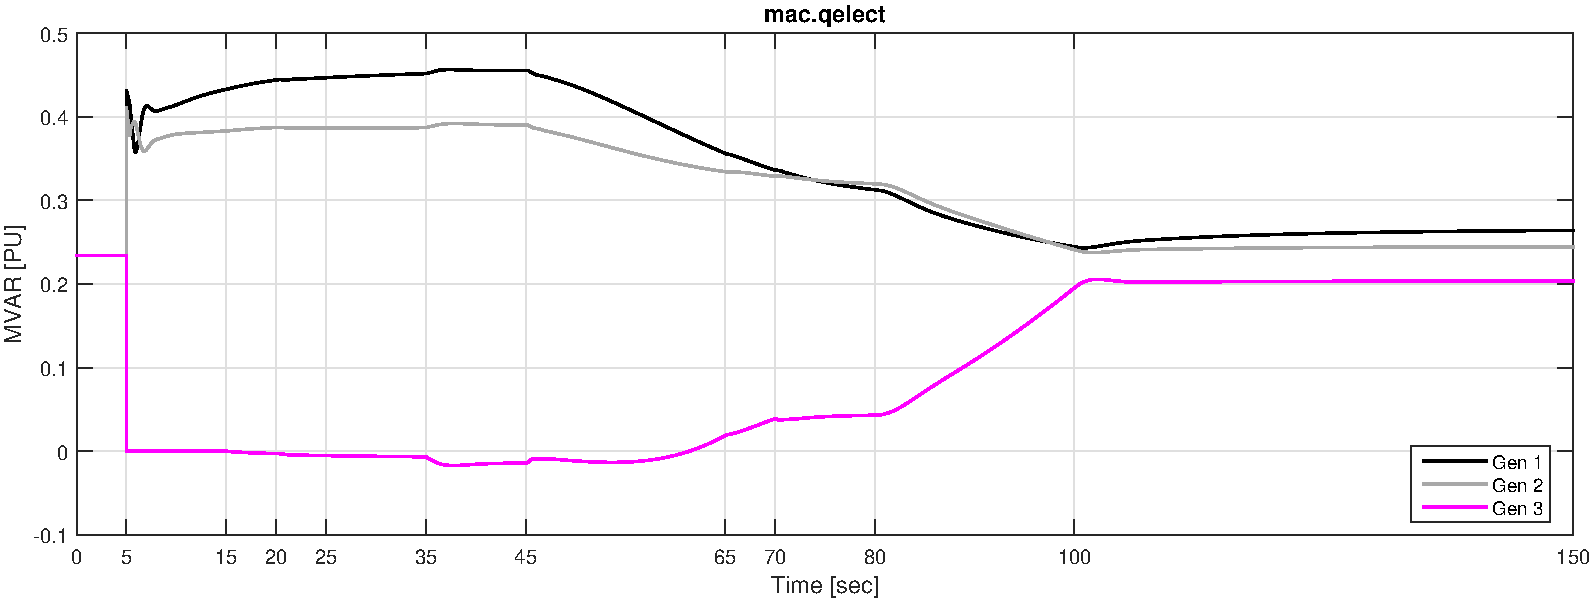
\includegraphics[width=\linewidth]{distinctQelect}

\pagebreak
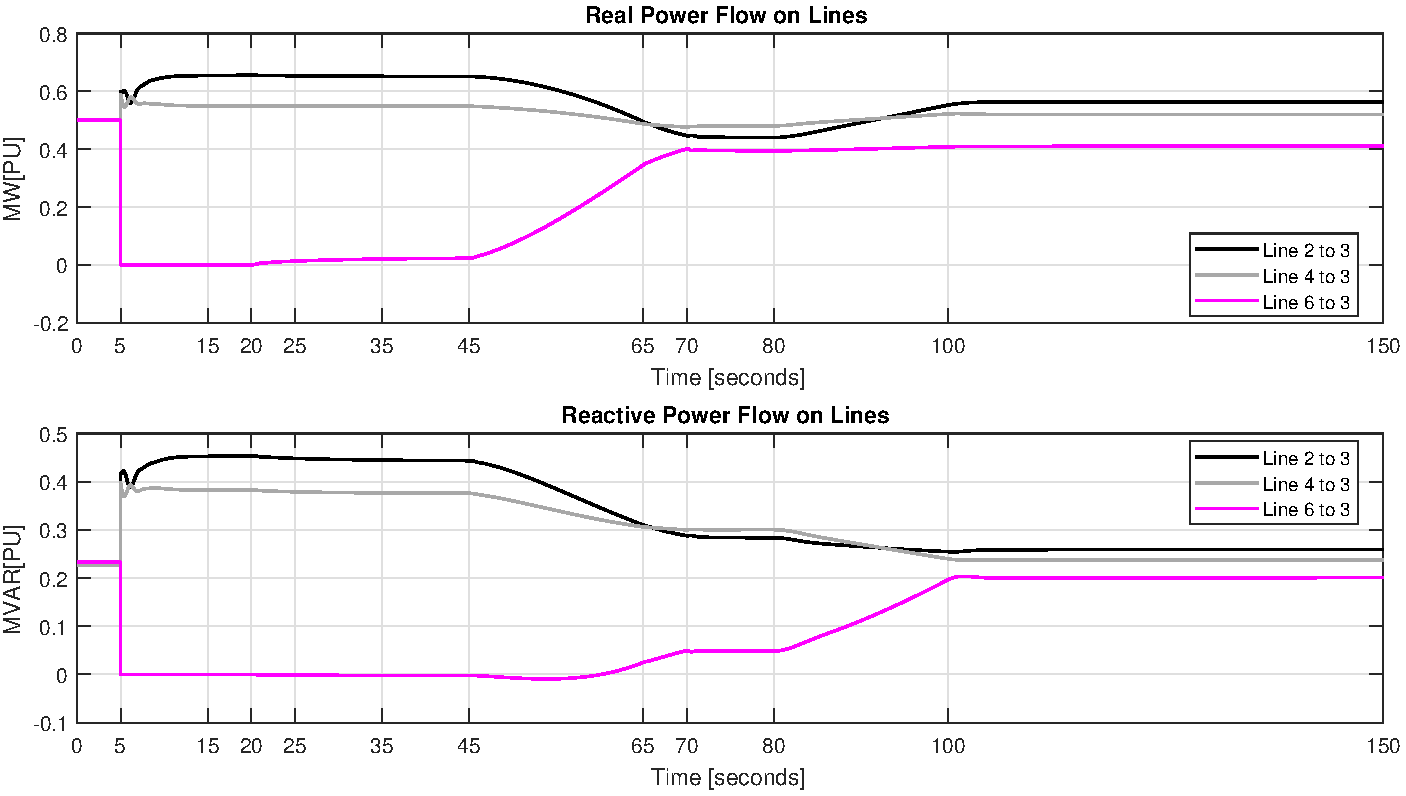
\includegraphics[width=\linewidth]{distinctLoadFlow}
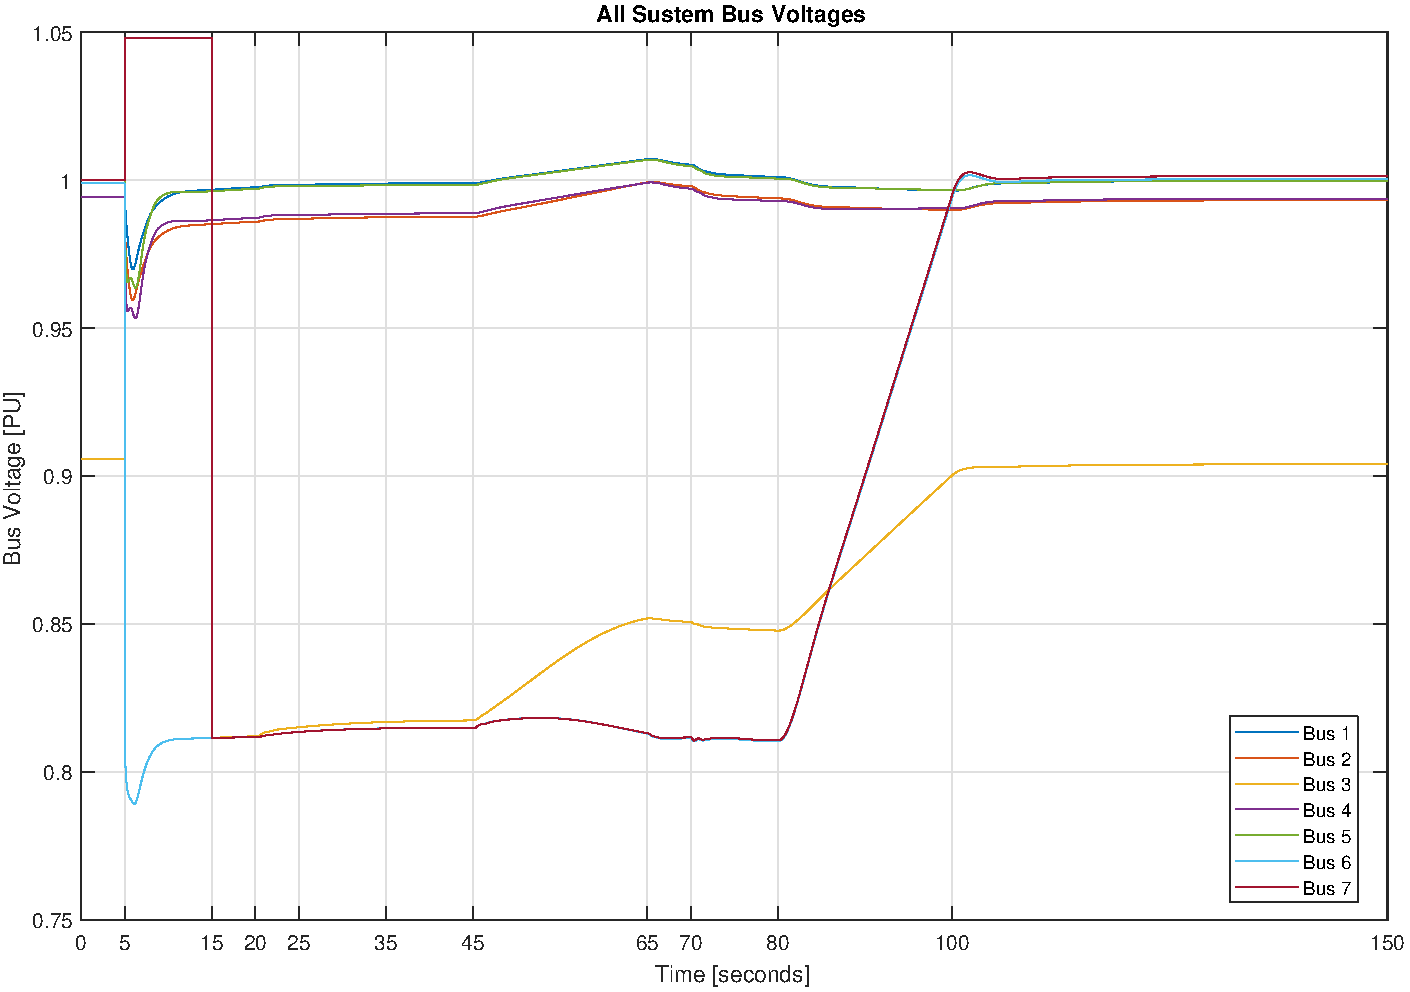
\includegraphics[width=\linewidth]{distinctBusV}


\pagebreak
\paragraph{Machine Trip Logic Code} \ \\
Most `un-trip' action takes place in the \verb|mac_trip_logic| file.
Such actions include:
\begin{itemize}
\item Trip generator 3
\item Set mechanical power to zero and bypass governor
\item Un-trip generator 3
\item Bypass exciter
\item Re-initialize machine
\item Re-init governor
\item Ramp governor R back 
\item Re-init and remove bypass on exciter
\item Ramp governor $P_{ref}$
\item Ramp exciter refernece
\end{itemize} 

It should be noted that the \verb|mac_trip_logic| routine usage was created `pre-global g', and as a result, passes variables in and out that are essentially globals.
Realistically, only a data index would need to be passed into the function, and any action can take place directly on the associated \verb|g.mac.mac_trip_states| vector or other required global.

\inputminted[
		frame=lines,
		framesep=2mm,
		baselinestretch=1.2,
		bgcolor=gray!13,
		fontsize=\footnotesize,
		linenos,
		breaklines
		]{MATLAB}% lang
		{../../../../PST/0-examples/unTrip/mac_trip_logic_Gen_3_G.m}% file name

\pagebreak
\paragraph{Turbine Governor Modulation Code} \ \\
The \verb|mtg_sig| file was used to ramp the governors $P_{ref}$  back to the original value.
\inputminted[
		frame=lines,
		framesep=2mm,
		baselinestretch=1.2,
		bgcolor=gray!13,
		fontsize=\footnotesize,
		linenos,
		breaklines
		]{MATLAB}% lang
		{../../../../PST/0-examples/unTrip/mtg_sig_PrefRamp.m}% file name
		
\end{document}